\section{Execution Time Prediction for Energy-Efficiency}
\label{sec:prediction}

\subsection{Overview}
\label{sec:prediction.overview}

%The main challenge in developing our prediction-based controller is determining how to predict the
%appropriate frequency to use for each job. The main source of execution time
%variation between jobs is due to different inputs and program state. Thus, we
%need a model to map job input and program state values to frequency
%levels. In general, finding a direct mapping from input values to frequency levels
%is challenging because the mapping can be irregular and complicated. In
%addition, this mapping varies from application to application. For example, for
%one application, pressing the ``down'' key may correspond to a large increase
%in execution time while for other applications it may have no effect on execution
%time. 
%As a result,
%we break the prediction down into multiple steps and take advantage of the
%program source to give us hints about how input values and program state will
%affect execution time.

% Control flow graph
\begin{figure}
  \begin{center}
    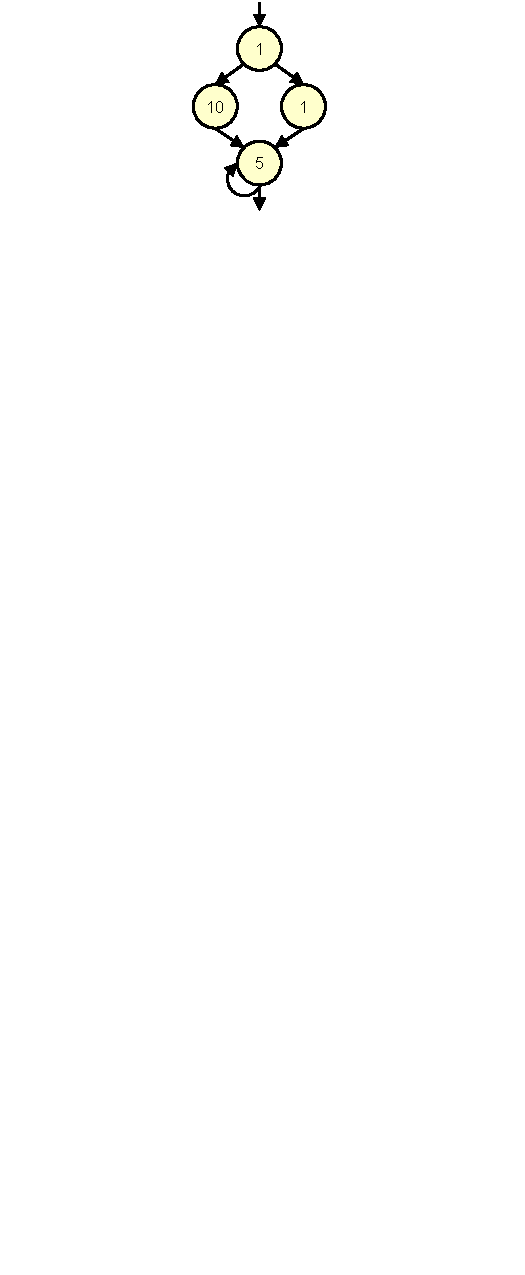
\includegraphics{exec_time_prediction/figs/cfg.pdf}
    \caption{Example control flow graph. Each node is annotated with its number of instructions.}
    \label{fig:prediction.cfg}
  \end{center}
\end{figure}

The basic intuition behind our prediction methodology is that, to first-order,
execution time correlates with the number of instructions run. Variations in
the number of instructions run are described by the control flow taken by a
specific job. For example, consider the control flow graph for a task shown in
Figure~\ref{fig:prediction.cfg}. Each node is marked with its number of instructions.
Taking the left branch instead of the right
branch corresponds to nine more instructions being executed. Similarly, each
additional loop iteration of the last basic block adds five instructions to the
number of instructions executed. By knowing which branch is taken and the
number of loop iterations, we can know the number of instructions
executed and estimate the execution time. 
With an estimate of the execution time, we can then estimate the performance-scaling impact of DVFS and choose
an appropriate frequency and voltage level to run at in order to just
meet the deadline.

% Prediction flow
\begin{figure}
  \begin{center}
    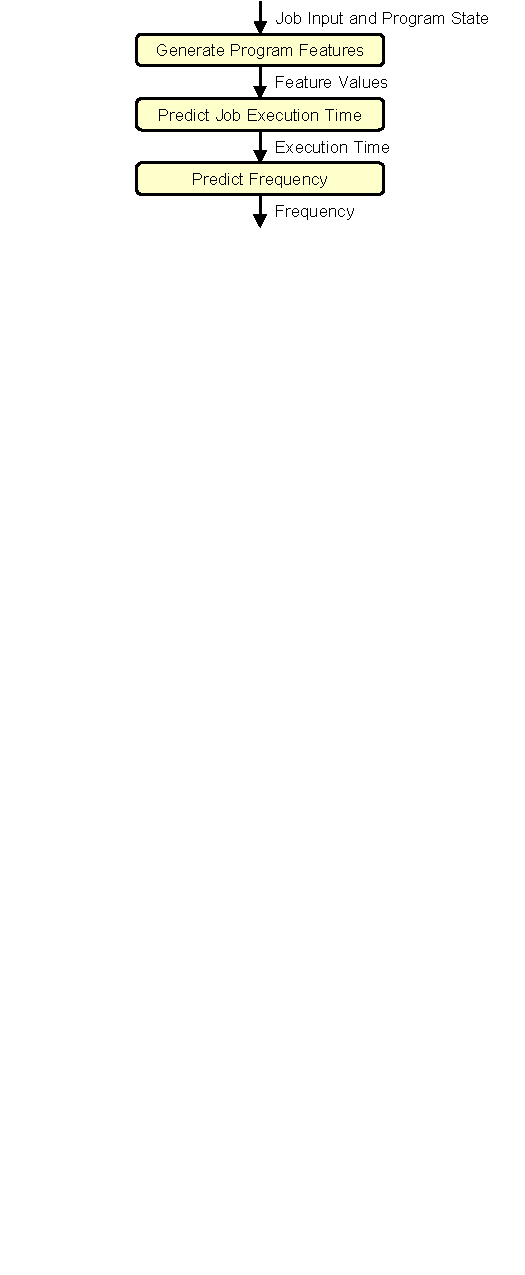
\includegraphics{exec_time_prediction/figs/prediction_flow.pdf}
    \caption{Steps to predict execution time from job input and program state.}
    \label{fig:prediction.prediction_flow}
  \end{center}
\end{figure}

Figure~\ref{fig:prediction.prediction_flow} shows the main steps in our
prediction method. We first instrument the task source code and use program
slicing to create a code fragment that will
calculate control flow features for a job. The code fragment is run before a
job executes in order to generate the control flow features
(Section~\ref{sec:prediction.features}). Next, we use a linear model, which we train off-line, to map
control flow features to an execution time estimate for the job 
(Section~\ref{sec:prediction.model}). Finally, we use classical linear models \cite{xie-pldi03, wu-micro05}
that describe the frequency-performance trade-off of DVFS to select an
appropriate frequency (Section~\ref{sec:prediction.dvfs}).

\subsection{Program Features}
\label{sec:prediction.features}

% Example insertion of feature counters
\begin{figure}
  \begin{center}
    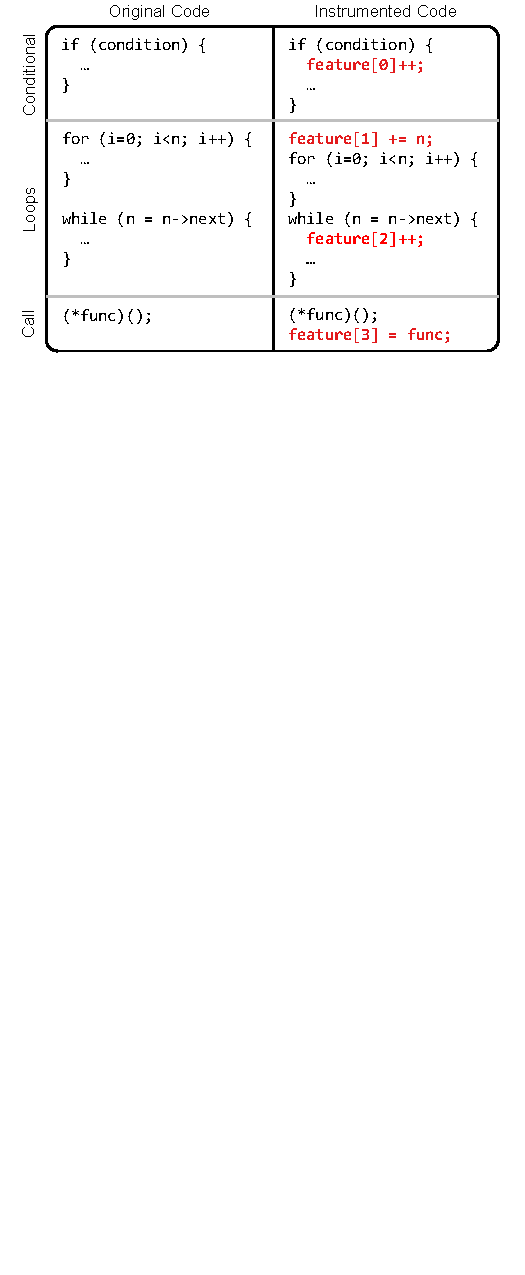
\includegraphics{exec_time_prediction/figs/features.pdf}
    \caption{Example of feature counters inserted for conditionals, loops, and function calls.}
    \label{fig:prediction.features}
  \end{center}
\end{figure}

The first step needed for our prediction is to generate control flow features.
That is, we want to know the control flow of a task when executing with a
specific input and program state.
For this purpose, we instrument the task source to count these control flow features.
Specifically, we instrument the task to count the following features:
\begin{itemize}
  \item Number of iterations for each loop
  \item Number of times each conditional branch is taken
  \item Address of each function pointer call
\end{itemize}
Figure~\ref{fig:prediction.features} shows examples of how these features are
instrumented. 
We focus on control flow features because these explain 
most of the execution time variation. However, other features, such as variable
values or memory accesses, could be included to improve the prediction
accuracy.

% Add loop counters, slice
\begin{figure*}
  \begin{center}
    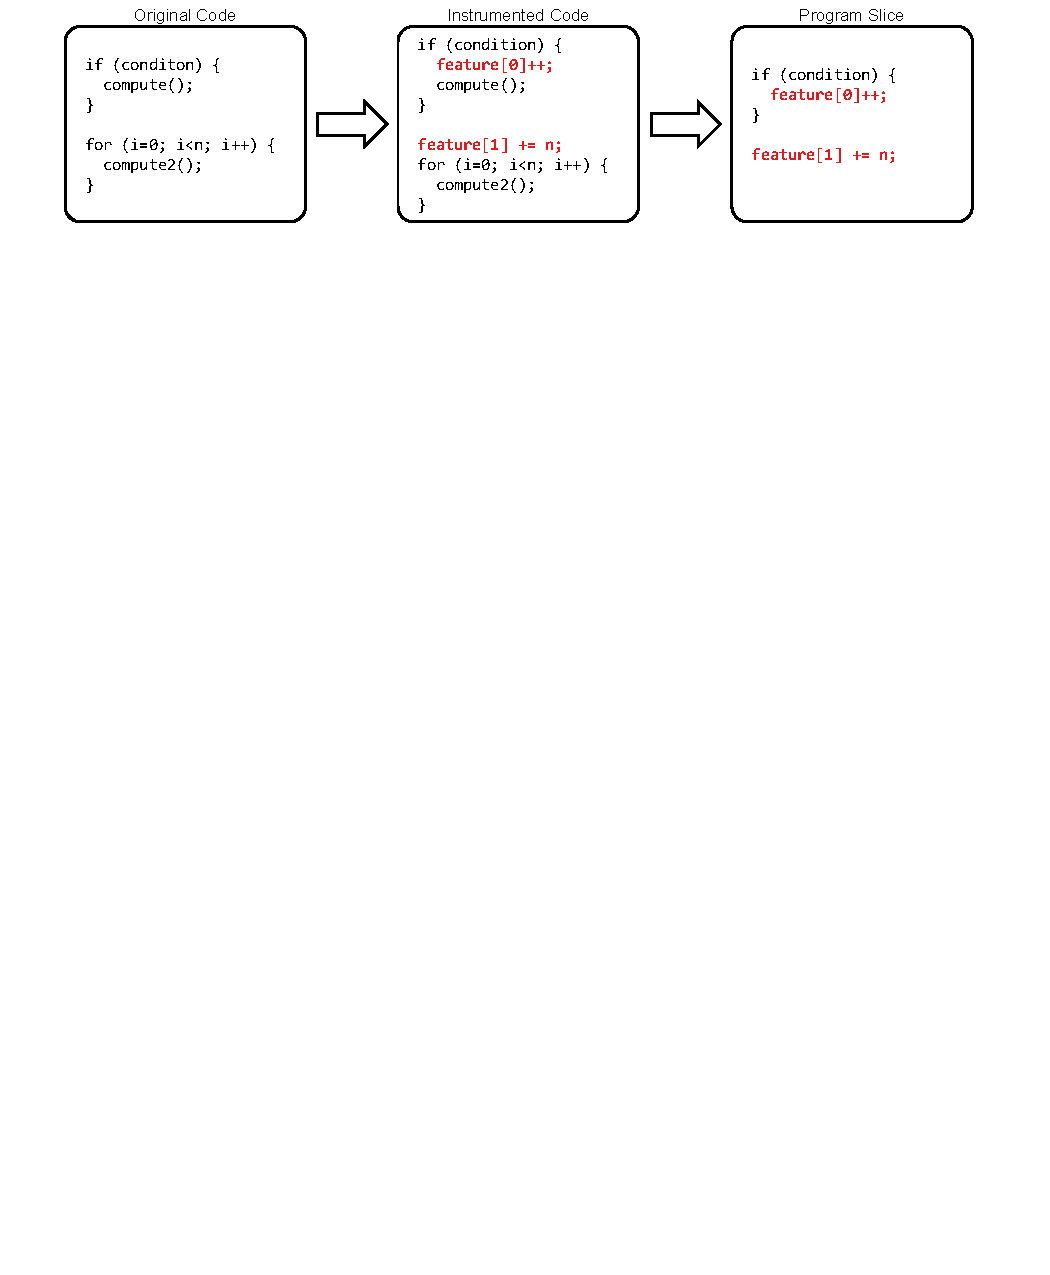
\includegraphics{exec_time_prediction/figs/code_transformations.pdf}
    \caption{Example of program slicing for control flow features.}
    \label{fig:prediction.code_transformations}
  \end{center}
\end{figure*}

Generating these features using an instrumented version of the task code is not
suitable for prediction because the instrumented task will take at least as long
as the original task to run. Instead, we need to quickly generate these features before
the task execution. In order to minimize the prediction execution time, we use
program slicing to produce the minimal code needed to calculate these features.
Figure~\ref{fig:prediction.code_transformations} shows a simple example of this
flow. By removing the actual computation and only running through the control
flow, the execution time can be greatly reduced. We refer to the resulting
program slice that computes the control flow
features as the \emph{prediction slice} or simply as the \emph{slice}.

One problem that arises with running this prediction slice before a task is the
issue of side-effects. That is, the slice could write to global variables and
break the correctness of the program. In order to prevent this, the slice
creates local copies of any global variables that are used. Values for these
local copies are updated at the start of the slice and writes are only applied
to the local copy. A similar process is applied to any arguments that are
passed by reference.

\subsection{Execution Time Prediction Model}
\label{sec:prediction.model}

% Runtime power of monitoring core
\begin{table}[tb]
  \begin{center}
    \begin{small}
    \begin{tabular}{|c|l|l|}

\hline
Variable & Type & Description \\ \hline\hline
$\bar{y}$ & Scalar & Predicted execution time \\ \hline
$\textbf{x}$ & Vector & Feature values \\ \hline
$\boldsymbol{\beta}$ & Vector & Model coefficients \\ \hline\hline
$\textbf{y}$ & Vector & Profiled execution times \\ \hline
$\textbf{X}$ & Matrix & Profiled feature values \\ \hline
$\textbf{X}\boldsymbol{\beta} - \textbf{y}$ & Vector & Prediction errors \\ \hline\hline
$\alpha$ & Scalar & Under-predict penalty weight \\ \hline
$\gamma$ & Scalar & Number of terms penalty weight \\ \hline
$\|\cdot\|$ & Scalar & L2-norm (sum of squares) \\ \hline
$\|\cdot\|_1$ & Scalar & L1-norm (sum of absolute values) \\ \hline

\end{tabular}


    \end{small}
    \caption{Variable and notation descriptions.}
    \label{tab:prediction.variables}
  \end{center}
\end{table}

Next, we need to predict the execution time from the control flow features.  This section
describes our model that maps features to execution time.
Table~\ref{tab:prediction.variables} summarizes the variables and
notation that are used in this section. 
We use a linear model to map features to execution time as this captures the
basic correlation. 
Higher-order or non-polynomial models may provide better accuracy.
However, a linear model has the advantage of being both simple to
train and fast to evaluate at run-time. In addition, it is always convex which
allows us to use convex optimization-based methods to fit the model.
Our linear model can be expressed as
\begin{align*}
  \bar{y} = \mathbf{x} \boldsymbol{\beta}
\end{align*}
where $\bar{y}$ is the predicted execution time, $\mathbf{x}$ is a vector of
feature values, and $\boldsymbol{\beta}$ are the coefficients that map feature
values to execution time. These $\boldsymbol{\beta}$ coefficients are
fit using profiling data. Specifically, we profile the program to
produce a set of training data consisting of execution times $\mathbf{y}$ and
feature vectors $\mathbf{X}$ (i.e., each row of $\mathbf{X}$ is a vector of
features, $\mathbf{x}_i$, for one job). Note that in order to achieve the expected linear
correlation between features and execution time, addresses recorded for
function calls are converted to a one-hot encoding indicating whether particular
function addresses were called or not.

The most common way to fit a linear model is to use linear least squares regression.
Linear least squares regression finds the coefficients $\boldsymbol{\beta}$ that minimize the mean
square error:
\begin{align*}
\begin{aligned}
  \underset{\boldsymbol{\beta}}{\text{argmin}} & & \|\mathbf{X}\boldsymbol{\beta} - \textbf{y}\|^2
\end{aligned}
\end{align*}
Essentially, this aims to minimize the sum of the absolute errors in the
prediction. That is, it weights negative and positive errors equally. However,
these two errors lead to different behaviors on our system.
Negative errors (under-prediction) lead to deadline misses since we predict the
job to run faster than its actual execution time. On the other hand, positive errors
(over-prediction) result in an overly conservative frequency setting which does
not save as much energy as possible. In order to maintain a good user
experience, we would prefer to avoid deadline misses, possibly at the cost of
energy usage. In other words, we should place greater weight on avoiding
under-prediction as opposed to over-prediction.

We can place greater weight on under-prediction by modifying our optimization objective:
\begin{align*}
\begin{aligned}
  \underset{\boldsymbol{\beta}}{\text{argmin}} & & \|pos(\textbf{X}\boldsymbol{\beta} - \textbf{y})\|^2 + \alpha \|neg(\textbf{X}\boldsymbol{\beta} - \textbf{y})\|^2
\end{aligned}
\end{align*}
where $pos(x) = max\{x, 0\}$ and $neg(x) = max\{-x, 0\}$ and these functions are applied
element-wise to vectors. Thus, $\|pos(\textbf{X}\boldsymbol{\beta} -
\textbf{y})\|^2$ represents the over-prediction error and
$\|neg(\textbf{X}\boldsymbol{\beta} - \textbf{y})\|^2$ represents the
under-prediction error. $\alpha$ is a weighting factor that allows us to place a
greater penalty on under-predictions by setting $\alpha > 1$.
Since this objective is convex, we can use existing convex optimization solvers
to solve for $\boldsymbol{\beta}$.

Coefficients which are zero imply that the corresponding control flow features
do not need to be calculated by the prediction slice. We can use this
information to further reduce the size and execution time of the prediction
slice. We can extend our optimization objective to favor using less features
by using the Lasso method \cite{lasso-jrss96}:
\begin{align*}
\begin{aligned}
  \underset{\boldsymbol{\beta}}{\text{argmin}} & & \|pos(\textbf{X}\boldsymbol{\beta} - \textbf{y})\|^2 + \alpha \|neg(\textbf{X}\boldsymbol{\beta} - \textbf{y})\|^2 + \gamma \|\boldsymbol{\beta}\|_1
\end{aligned}
\end{align*}
where $\|\cdot\|_1$ is the L1-norm and $\gamma$ is a weighting factor that
allows us to trade-off prediction accuracy with the number of features needed.

\subsection{DVFS Model}
\label{sec:prediction.dvfs}

% DVFS linearity
\begin{figure}
  \begin{center}
    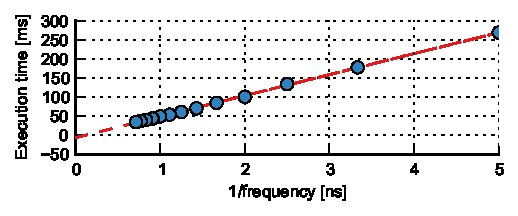
\includegraphics{exec_time_prediction/figs/dvfs_linearity.pdf}
    \caption{Average execution time of jobs (frames) for ldecode (video
    decoding) as frequency level varies.}
    \label{fig:prediction.dvfs_linearity}
  \end{center}
\end{figure}

Given a predicted execution time, we need to
estimate how the execution time will change with varying frequency. For this,
we use the classical linear model found in literature \cite{xie-pldi03, wu-micro05}:
\begin{align*}
  t = T_{mem} + N_{dependent}/f
\end{align*}
where $t$ is the execution time, $T_{mem}$ is the memory-dependent execution time
that does not scale with frequency, $N_{dependent}$ is the number of CPU cycles
that do not overlap with memory and scale with frequency, and $f$ is
the frequency.
In order to verify this linearity assumption, we measured average job execution
times as frequency was varied. Figure~\ref{fig:prediction.dvfs_linearity} shows
the average job execution time versus $1/f$ for ldecode (video decoder
application). We can see that $t$ and $1/f$ do show a linear relationship. We
saw similar results for the other applications we tested.

For this linear model, by predicting the execution time at two points, we can
determine $T_{mem}$ and $N_{dependent}$ 
for a job and calculate the minimum frequency $f$ to satisfy a
given time budget $t_{budget}$. More specifically, we predict the execution time
$\bar{t}_{fmin}$ at minimum frequency $f_{min}$ and the execution time
$\bar{t}_{fmax}$ at maximum frequency $f_{max}$. Using these two points, we can calculate $T_{mem}$ and $N_{dependent}$ as
\begin{align*}
  N_{dependent} &= \frac{f_{min}f_{max}(\bar{t}_{fmin} - \bar{t}_{fmax})}{f_{max} - f_{min}} \\
  T_{mem} &= \frac{f_{max}\bar{t}_{fmax} - f_{min}\bar{t}_{fmin}}{f_{max} - f_{min}}
\end{align*}

For a given budget $t_{budget}$, we want the minimum frequency $f_{budget}$ that will meet this time. This can be calculated as
\begin{align*}
  f_{budget} = \frac{N_{dependent}}{t_{budget} - T_{mem}}
\end{align*}

Since execution time can vary even with the same job inputs and program state, 
we add a margin to the predicted execution times used
($t_{fmin}$ and $t_{fmax}$). In our experiments we used a margin of 10\%. A
higher margin can decrease deadline misses while a lower margin can improve the
energy savings. 
The resulting predicted frequency is the exact frequency that we expect will just satisfy the
time budget. However, DVFS is only supported for a set of
discrete frequency levels. Thus, the actual frequency we select is the smallest
frequency allowed that is greater than $f_{budget}$. 

% Effective budget
\begin{figure}
  \begin{center}
    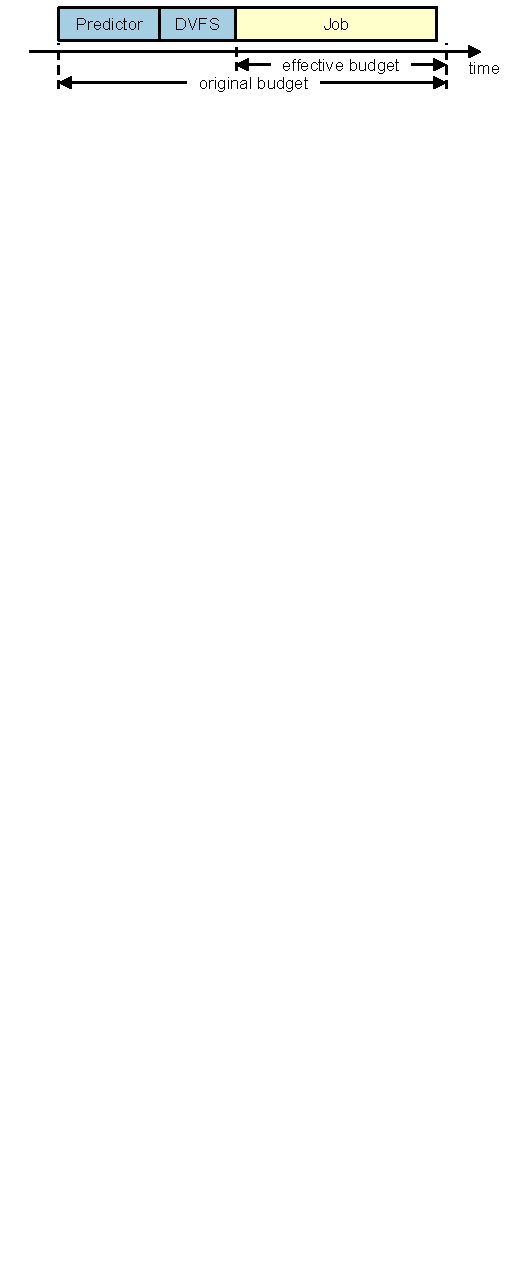
\includegraphics{exec_time_prediction/figs/effective_budget.pdf}
    \caption{The effective budget decreases due to slice and DVFS execution time.}
    \label{fig:prediction.effective_budget}
  \end{center}
\end{figure}

% DVFS switching time
\begin{figure}
  \begin{center}
    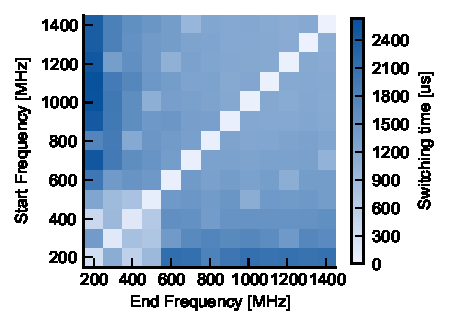
\includegraphics{exec_time_prediction/data/dvfs_heatmap.pdf}
    \caption{95th-percentile switching times for DVFS.}
    \label{fig:prediction.dvfs_heatmap}
  \end{center}
\end{figure}

The execution of the prediction slice and DVFS switch
reduces the amount of time available for a job to execute and still satisfy its
budget. Thus, the effective budget when choosing a frequency to run at
needs to consider these overheads (see
Figure~\ref{fig:prediction.effective_budget}). Although the execution time of
the prediction slice can be measured, the DVFS switching time must be
estimated, as the switch has not been performed yet.  This is done by
microbenchmarking the DVFS switching time.
Figure~\ref{fig:prediction.dvfs_heatmap} shows the 95th-percentile DVFS
switching times for our test platform for each possible start and ending
frequency. We use the 95th-percentile switching times in order to be
conservative in our estimate of DVFS switching time while omitting rare
outliers. 
%As the switching time depends on the start and end frequencies, we
%search through the target frequencies to find the minimal frequency that will
%satisfy the time budget, taking into account the slice and DVFS times.

% If the portion of the job that does not scale with frequency is negligible
% (i.e., $T_{mem} \approx 0$), then we only need to profile at one point and
% $N_{dependent}$ simplifies to
% \begin{align*}
%   N_{dependent} &= t_{fmax}f_{max}
% \end{align*}
% and the frequency calculation simplifies to
% \begin{align*}
%   f_{deadline} = \frac{N_{dependent}}{t_{deadline}} = \frac{t_{fmax}f_{max}}{t_{deadline}}
% \end{align*}
% For the applications we tested, we found $T_{mem}$ to be negligible. Thus, we
% were able to select an appropriate DVFS level with only one predicted execution
% time (at $f_{max}$).

\subsection{Alternate Prediction Models}

In this section, we have described our specific prediction strategy for each
step in our overall prediction flow shown in
Figure~\ref{fig:prediction.prediction_flow}. However, we note that each step in
this prediction flow can be substituted with alternate models as long as it
produces the needed prediction for the next step.
The most obvious change would be to use more complex prediction models for each
step (e.g., more features generated and higher-order, non-linear models).
For the benchmarks we evaluated, we saw relatively little gain to be had from
improved prediction (see Section~\ref{sec:evaluation.overheads}) and thus the
increased overheads of more complex models were not justified.
Instead, we discuss here some alternative extensions.

For feature generation, we have focused on automated generation in order for
the approach to be general and limit the need for domain-specific expertise.
However, this does not preclude the programmer from manually adding ``hints''
that they expect would correlate well with a job's execution time. For example,
the programmer may be able to extract meta-data from input files and manually
encode these to features.

%For our prediction-based DVFS controller, we focused on control flow features
%as these describe most of the execution time variation. Additional features may
%improve prediction accuracy for certain applications. For example,
%cache-sensitive applications may want to include features related to memory
%accesses. For multi-threaded applications, number of threads and features
%related to possible parallelism could be useful. In addition, the programmer
%could add ``hint'' features that they expect would correlate well with a
%job's execution time. For example, if they know that certain user inputs will
%correlate to high execution time, they could explicitly code these as features
%in the prediction slice.

One interesting extension to execution time prediction involves its use in
feature selection. Additional constraints could be added to the execution
time prediction in order to limit the use of features which require high
overhead to generate. Features over some overhead threshold could
be explicitly disallowed or the overhead for each feature could be
introduced as penalties in the optimization objective.
%For execution time prediction, many options exist including higher-order, non-linear
%models or machine-learning based approaches such as artificial neural networks.
% However, these approaches introduce both increased training time and on-line
% execution times. As this time reduces the effective deadline, the improvement
% in prediction accuracy needs to be large enough to justify the overhead.

The last step in our flow focuses on selecting an appropriate
frequency level for DVFS control. However, this last step could be substituted to
support other performance-energy trade-off mechanisms, such as heterogeneous
cores. By using alternate models for how the execution time scales with the
performance-energy trade-off mechanism, an appropriate operating point can be
selected for the mechanism of interest.
